\documentclass[12pt]{article}
\usepackage{graphics}
\usepackage[top=1in,bottom=1in,left=1in,right=1in]{geometry}
\usepackage{alltt}
\usepackage{array}	
\usepackage{graphicx}
\usepackage{tabularx}
\usepackage{verbatim}
\usepackage{setspace}
\usepackage{listings}
\usepackage{ulem}
\usepackage{tikz}
\usepackage{xcolor}

\usepackage{amssymb,amsmath, amsthm}
\usepackage{zed-csp}
\usepackage[cc]{titlepic}

\definecolor{codegreen}{rgb}{0,0.6,0}
\definecolor{codegray}{rgb}{0.5,0.5,0.5}
\definecolor{codepurple}{rgb}{0.58,0,0.82}
\definecolor{backcolour}{rgb}{0.95,0.95,0.92}

\lstdefinestyle{mystyle}{
    backgroundcolor=\color{backcolour},   
    commentstyle=\color{codegreen},
    keywordstyle=\color{magenta},
    numberstyle=\tiny\color{codegray},
    stringstyle=\color{codepurple},
    basicstyle=\ttfamily\footnotesize,
    breakatwhitespace=false,         
    breaklines=true,                 
    captionpos=b,                    
    keepspaces=true,                 
    numbers=left,                    
    numbersep=5pt,                  
    showspaces=false,                
    showstringspaces=false,
    showtabs=false,                  
    tabsize=1,
}

\lstset{style=mystyle}

\title{SOEN 331 - S: Formal Methods\\for Software Engineering\\
\ \\
Assignment 1}
\author{Nathan Grenier, Nirav Patel}
\date{\today}
\begin{document}
\begin{spacing}{1.5}
	\maketitle
	\thispagestyle{empty}
							    
	\newpage
							    
	\pagenumbering{arabic}
							    
	\section*{PROBLEM 1: Propositional logic (5 pts)}
												
	You are shown a set of four cards placed on a table, each of which has a \textbf{number} on one
	side and a \textbf{color} on the other side. The visible faces of the cards show the numbers \textbf{9} and
	\textbf{11}, and the colors \textbf{blue}, and \textbf{yellow}.\\
												
	Which card(s) must you turn over in order to test the truth of the proposition that “\textit{If
		the face of a card is \textbf{blue}, then it has a \textbf{prime} number on the other side}”? Explain your
	reasoning by deciding for \uline{each} card whether or not it should be turned over and why.\\
												
	\textbf{Solution}: The proposition states: "If the face of a card is \textbf{blue}, then it has a \textbf{prime} number on the other side."\\
												
	Given the cards with visible faces showing \textbf{9}, \textbf{11}, \textbf{blue}, and \textbf{yellow}, we need to determine which cards to turn over to test this proposition.\\
												
	We will apply propositional logic to decide which cards to flip:
												
	\begin{enumerate}
		\item If a card has a \textbf{prime} number on one face, we do not need to turn it over. The face having a \textbf{prime} number is not exclusive to blue cards. The "Denying the Antecedent" fallacy should be avoided.
		\item If a card has a \textbf{non-prime} number on one face, and it is \textbf{blue}, we must turn it over to ensure it contradicts the proposition. This would verify the "Modus Tollens" rule of inference.
		\item If a card has a \textbf{blue} color on one face, we must turn it over to ensure it has a \textbf{prime} number on the other side. This would verify the "Modus Ponens" rule of inference.
		\item If a card has a \textbf{non-blue} color on one face, we do not need to turn it over, as it does not contradict the proposition. The "Affirming the Antecedent" should be avoided. \\
	\end{enumerate}
												
	Now, let's analyze each card:
	\begin{enumerate}
		\item The card showing \textbf{9} should be turned over since it is a non-prime number. If it's flipped side is blue, it would violate the proposition.
		\item The card showing \textbf{11} does not need to be turned over, as the proposition makes no claim regarding non-prime numbers.
		\item The card showing \textbf{blue} must be turned over to verify if it has a prime number on the other side, as per the proposition.
		\item The card showing \textbf{yellow} does not need to be turned over because the proposition only concerns cards with blue faces.\\
	\end{enumerate}
												
	Therefore, we must turn over the card with the \textbf{blue} and \textbf{non-prime} number on the other side to test the proposition. $\therefore$
												
	\newpage
												
								
	\newpage
							    
	\section*{PROBLEM 2: Predicate logic (14 pts)}
												
	\textbf{Part 1} (8 pts)\\
	Consider types \textit{Object}, and the binary relation Orbits over the domain of all celestial objects,
	which is codified by clause \texttt{object/1} in Prolog (available in \texttt{solar.pl}):
											
	\begin{enumerate}
		\item 
		      (2 pts) Construct a formula in predicate logic to define a planet, where planet is defined
		      as an object whose mass is greater than or equal to $0.33\times10^{24}$ \textit{KG}, and which it orbits around the
		      sun. For all practical purposes, you may ignore the $10^{24}$ \textit{KG} factor.\\

		      \textbf{Solution}: To define a planet in predicate logic based on its mass and orbit properties, we can construct the following formula:

		      \begin{itemize}
		      	\item Let $P(x)$ represent "$x$ is a planet."
		      	\item Let $M(x)$ represent "$x$ has a mass greater than 0.33 KG."
		      	\item Let $O(x,y)$ represent "$x$ orbits around $y$."
		      	\item Let $S$ represent the sun.
		      	      
		      \end{itemize}

		      The formula to define a planet can be expressed as:
		      $$P(x)\equiv (M(x) \land O(x, S))$$

		      This formula states that an object $x$ is considered a planet if it has a mass greater than 0.33 KG and orbits around the sun. $\therefore$ \\

		      Use the formula for \textit{Planet} to construct a formula that defines the binary relation
		      \textit{is\_satellite\_of} in terms of the binary relation \textbf{Orbits}. A satellite is an object that orbits around a planet.\\

		      \textbf{Solution}: To define the binary relation "is satellite of" in terms of the binary relation "Orbits," where a satellite is an object that orbits around a planet, we can construct the following formula:

		      \begin{itemize}
		      	
		      	\item Let $S(x,y)$ represent "$x$ is a satellite of $y$."
		      	\item Let $P(x)$ represent "$x$ is a planet."
		      	\item Let $O(x,y)$ represent "$x$ orbits around $y$."
		      	      
		      \end{itemize}

		      The formula to define a satellite in terms of the Orbits relation can be expressed as:
		      $$S(x,y) \equiv O(x,y) \land P(y)$$
		      		      		              
		\item 
		      (3 pts) (\uline{\textbf{PROGRAMMING}}) Map your formulas to Prolog rules \texttt{is\_planet/1}, and
		      \texttt{is\_satellite\_of/2}, and demonstrate how it works by executing both ground- and
		      non-ground queries. \textbf{Identify the type of each query}.\\

		      \textbf{Solution}: We can define the following Prolog rules based on the given predicates:

		      \begin{lstlisting}
% Rule to define a planet
is_planet(X) :- mass(X, Mass), Mass >= 0.33, orbits(X, sun).

% Rule to define a satellite of a planet
is_satellite_of(Satellite, Planet) :- is_planet(Planet), orbits(Satellite, Planet).       
		      \end{lstlisting}

		      Now, we demonstrate how these rules work using both ground and non-ground queries:\\

		      \textbf{Ground Queries}:

		      \begin{enumerate}
		      	\item 
		      	      Query \texttt{?- is\_planet(pluto).}
		      	      \begin{itemize}
		      	      	\item Type: Ground Query
		      	      	\item Result: \texttt{`false`}
		      	      \end{itemize}
		      	           
		      	\item 
		      	      Query \texttt{?- is\_planet(mars).}
		      	      \begin{itemize}
		      	      	\item Type: Ground Query
		      	      	\item Result: \texttt{`true`}
		      	      \end{itemize}
		      	           
		      	\item 
		      	      Query \texttt{?- is\_satellite\_of(moon, earth).}
		      	      \begin{itemize}
		      	      	\item Type: Ground Query
		      	      	\item Result: \texttt{`true`}\\
		      	      \end{itemize}
		      \end{enumerate}
		      		      		      		      		      		      		      		      		      
		      \textbf{Non-Ground Queries}:
		      \begin{enumerate}
		      	 	
		      	\item 
		      	      Query \texttt{?- is\_planet(P).}
		      	      \begin{itemize}
		      	      	\item Type: Non-Ground Query
		      	      	\item Result: \texttt{\\
		      	      		P = mercury;\\
		      	      		P = venus;\\
		      	      		P = earth;\\
		      	      		P = mars;\\
		      	      		P = jupiter;\\
		      	      		P = saturn;\\
		      	      		P = uranus;\\
		      	      		P = neptune;\\
		      	      	false}
		      	      \end{itemize}
		      	           
		      	\item 
		      	      Query \texttt{?- is\_satellite\_of(S, mars).}
		      	      \begin{itemize}
		      	      	\item Type: Non-Ground Query
		      	      	\item Result: \texttt{\\
		      	      		S=deimos;\\
		      	      		S=phobos;\\
		      	      	false\\}\\
		      	      \end{itemize}

                \item
                    Query \texttt{?- is\_satellite\_of(moon, Planet).}
                    \begin{itemize}
                        \item Type: Non-Ground Query
                        \item Result: \texttt{\\
                            Planet = earth;\\
                            false\\}
                    \end{itemize}
		      	              
		      \end{enumerate}
		      		      		      		      		      		      		      		      
		\item
		      (3 pts) (\uline{\textbf{PROGRAMMING}}) Construct a Prolog rule \texttt{obtain\_all\_satellites/2}
		      that succeeds by returning a collection of all satellites of a given planet.\\
		      		      		      		      		      		      		      		      
		      \textbf{Solution}: We can define a rule named \texttt{all\_satellites/2} that collects all the satellites of a specified planet. The following describes an example of how the rule can be implemented:\\
		      		      		      		      		      		      		      		      
		      \begin{lstlisting}
% Rule to obtain all satellites of a given planet
all_satellites(Planet, Satellites) :- findall(Satellite, is_satellite_of(Satellite, Planet), Satellites).
		      \end{lstlisting}
		      		      		      		      		      		      		      		      
		      In this rule:
		      \begin{itemize}
		      	\item \texttt{Planet} is the input parameter representing the planet for which we want to           find its satellites.
		      	       
		      	\item \texttt{Satellites} is the output parameter that will contain a collection of all satellites of the specified planet.
		      	       
		      	\item \texttt{findall/3} is used to collect all solutions for \texttt{Satellite} that satisfy the condition \texttt{is\_satellite\_of(Satellite, Planet)}.
		      \end{itemize}
		      		      		      		      		      		      		      		      
		      We can test this rule using the following query:
		      		      		      		      		      		      		      		      
		      \textbf{Query}:\\
		      \texttt{?- all\_satellites(jupiter, Satellites).}
		      		      		      		      		      		      		      		      
		      \textbf{Result}:\\
		      \texttt{Satellites = [arche, callisto, europa, io, themisto]}\\
	\end{enumerate}
								
	\noindent \textbf{Part 2: Categorical propositions} (2 pts)\\
	In the domain of all integers, let $number(x)$ denote the statement “$x$ is a number”, and $composite(x)$ denote the statement “$x$ is a composite.” Formalize the following sentences and indicate their corresponding formal type.\\
							
	\textbf{Solution}: We will use the predicates number(x) and composite(x), and their corresponding formal types (A, E, I, O) to formalize the sentences.
								
	\begin{enumerate}
		\item "Some numbers are not composite."
		      		      		      		      		      		      		      
		      \begin{itemize}
		      	\item Formalization: $\exists x(number(x) \land \neg composite(x))$
		      	\item Corresponding Formal Type: O (Particular Negative)
		      \end{itemize}
		      		      		      		      		      		      		        
		\item "No numbers are prime."
		      		      		      		      		      		      		      
		      \begin{itemize}
		      	\item Formalization: $\forall x (number(x) \rightarrow composite(x))$
		      	\item Corresponding Formal Type: A (Universal Affirmative)
		      \end{itemize}
		      		      		      		      		      		      		        
		\item "Some numbers are not prime."
		      		      		      		      		      		      		      
		      \begin{itemize}
		      	\item Formalization: $\exists x(number(x) \land composite(x))$
		      	\item Corresponding Formal Type: I (Particular Affirmative)
		      \end{itemize}
		      		      		      		      		      		      		        
		\item "All numbers are prime."
		      		      		      		      		      		      		      
		      \begin{itemize}
		      	\item Formalization: $\forall x(number(x) \rightarrow \neg composite(x))$
		      	\item Corresponding Formal Type: E (Universal Negative) \\ \\ \\ \\
		      \end{itemize}
		      		      		      		      		      		      		              
	\end{enumerate}
							
	\noindent \textbf{Part 3: Categorical propositions} (4 pts)\\
	For subject $S$ and predicate $P$, we can express the Type $A$ categorical proposition as
							
	$$\forall s : S | s \in P$$
							
	\begin{enumerate}
		\item Prove formally that negating $A$ is logically equivalent to obtaining $O$ (and vice versa).
		      		      		      		      		      		      		      
		      \textbf{Solution}: We first determine the negation of $A$ ($\neg A$):
		      		      		      		      		      		      		      
		      $$\neg A = \neg (\forall s : S | s \in P ) = \exists s : S | s \notin P$$
		      		      		      		      		      		      		      
		      The equivalent expression obtained from determining the negation of $A$ is logically equivalent to the formulation of $O$. Similarly, we can obtain an $A$-type proposition using the negation of $O$:
		      		      		      		      		      		      		      
		      $$\neg (\exists s : S | s \notin P) = \forall s : S | s \in P$$
		      		      		      		      		      		      		      
		      We have therefore proven that negating $A$ is logically equivalent to obtaining $O$, and vice-versa.
		      		      		      		      		      		      		              
		\item Prove formally that negating E is logically equivalent to obtaining $I$ (and vice versa).
		      		      		      		      		      		      		      
		      \textbf{Solution}: We first determine the negation of $E$ ($\neg E$):
		      		      		      		      		      		      		      
		      $$\neg (\forall s : S | s \notin P)=\exists s : S | s \in P$$
		      		      		      		      		      		      		      
		      The equivalent expression obtained from determining the negation of $E$ is logically equivalent to the formulation of $I$. Similarly, we can obtain an $E$-type proposition using the negation of $I$:
		      		      		      		      		      		      		      
		      $$\neg (\exists s : S | s \in P) = \forall s : S | s \notin P$$
		      		      		      		      		      		      		      
		      We have therefore proven that negating $E$ is logically equivalent to obtaining $I$, and vice-versa.
		      		      		      		      		      		      		      
	\end{enumerate}
								    
							    
	\newpage
							    
	\section*{PROBLEM 3: Temporal logic (22 pts)}
							
	\textbf{Part 1} (16 pts)\\
							    
	The behavior of a program is expressed by the following temporal formula:
							
	\begin{figure}[htp]
		\centering
		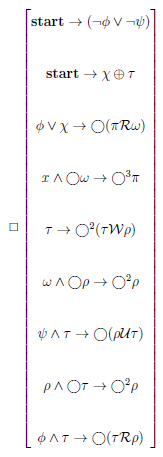
\includegraphics{static/templogicfigure.png}
		\caption{Temporal Formula}
		\label{fig:figure}
	\end{figure}
							
    \newpage
							
	\begin{enumerate}
		\item (9 pts) Visualize all models of behavior.\\
		      \textbf{Solution}:\\
		      \begin{center}
		      	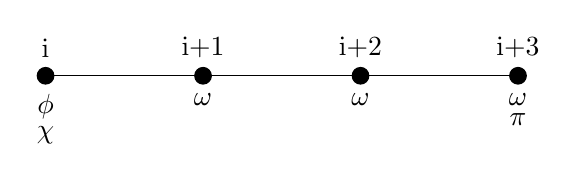
\begin{tikzpicture}
		      			    
		      		\draw (1,0) -- (7,0); 
		      		   
		      		\filldraw (1,0) circle (3pt) node[below=3pt] {\shortstack{$\phi$\ \\ $\chi$}} node[above=3pt] {i};
		      		\filldraw (3,0) circle (3pt) node[below=3pt] {\shortstack{$\omega$}} node[above=3pt] {i+1};
		      		\filldraw (5,0) circle (3pt) node[below=3pt] {\shortstack{$\omega$}} node[above=3pt] {i+2};
		      		\filldraw (7,0) circle (3pt) node[below=3pt] {\shortstack{$\omega$ \\ $\pi$}} node[above=3pt] {i+3};

		      	\end{tikzpicture}t

		      	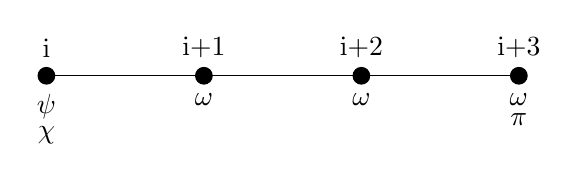
\begin{tikzpicture}
		      			
		      		\draw (1,0) -- (7,0); 
		      		   
		      		\filldraw (1,0) circle (3pt) node[below=3pt] {\shortstack{$\psi$\ \\ $\chi$}} node[above=3pt] {i};
		      		\filldraw (3,0) circle (3pt) node[below=3pt] {\shortstack{$\omega$}} node[above=3pt] {i+1};
		      		\filldraw (5,0) circle (3pt) node[below=3pt] {\shortstack{$\omega$}} node[above=3pt] {i+2};
		      		\filldraw (7,0) circle (3pt) node[below=3pt] {\shortstack{$\omega$ \\ $\pi$}} node[above=3pt] {i+3};
		      		  
		      	\end{tikzpicture}t

		      	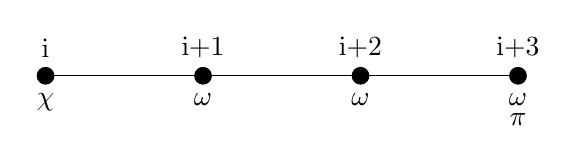
\begin{tikzpicture}

		      		\draw (1,0) -- (7,0); 
		      		   
		      		\filldraw (1,0) circle (3pt) node[below=3pt] {\shortstack{$\chi$}} node[above=3pt] {i};
		      		\filldraw (3,0) circle (3pt) node[below=3pt] {\shortstack{$\omega$}} node[above=3pt] {i+1};
		      		\filldraw (5,0) circle (3pt) node[below=3pt] {\shortstack{$\omega$}} node[above=3pt] {i+2};
		      		\filldraw (7,0) circle (3pt) node[below=3pt] {\shortstack{$\omega$ \\ $\pi$}} node[above=3pt] {i+3};
		      		  
		      	\end{tikzpicture}t

		      	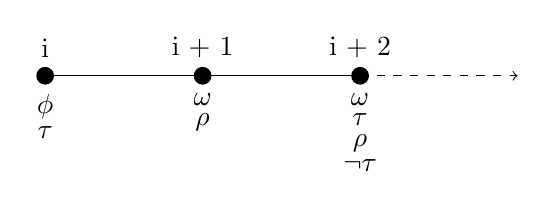
\begin{tikzpicture}
		      		\draw (1,0) -- (5,0);
		      		\filldraw (1,0) circle (3pt) node[below=3pt] {\shortstack{$\phi$ \\ $\tau$}} node[above=3pt] {i};
		      		\filldraw (3,0) circle (3pt) node[below=3pt] {\shortstack{$\omega$ \\ $\rho$}} node[above=3pt] {i + 1};
		      		\filldraw (5,0) circle (3pt) node[below=3pt] {\shortstack{$\omega$ \\ $\tau$ \\ $\rho$ \\ $\neg \tau$}} node[above=3pt] {i + 2};
		      		  
		      		\draw[dashed, ->] (5,0) -- (7,0);
		      	\end{tikzpicture}t

		      	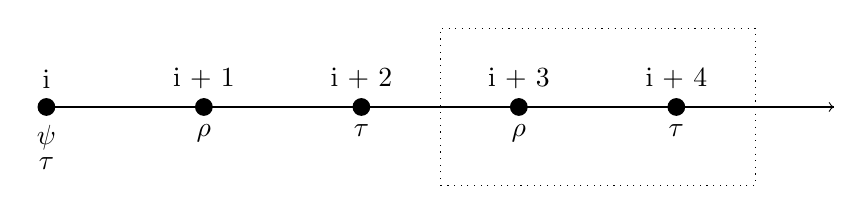
\begin{tikzpicture}
		      		\draw (1,0) -- (11,0);
		      		   
		      		\filldraw (1,0) circle (3pt) node[below=3pt] {\shortstack{$\psi$ \\ $\tau$}} node[above=3pt] {i};
		      		\filldraw (3,0) circle (3pt) node[below=3pt] {\shortstack{$\rho$}}
		      		node[above=3pt] {i + 1};
		      		\filldraw (5,0) circle (3pt) node[below=3pt] {\shortstack{$\tau$}}
		      		node[above=3pt] {i + 2};
		      		\filldraw (7,0) circle (3pt) node[below=3pt] {\shortstack{$\rho$}}
		      		node[above=3pt] {i + 3};
		      		\filldraw (9,0) circle (3pt) node[below=3pt] {\shortstack{$\tau$}}
		      		node[above=3pt] {i + 4};

		      		\draw[dotted] (6,-1) rectangle (10,1);

		      		\draw[dashed, ->] (9,0) -- (11,0);
		      	\end{tikzpicture}t

		      	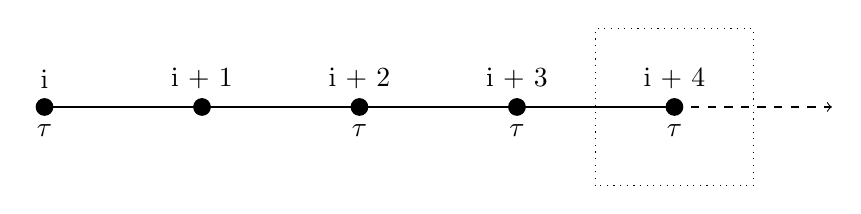
\begin{tikzpicture}
		      		\draw (1,0) -- (9,0);

		      		\filldraw (1,0) circle (3pt) node[below=3pt] {\shortstack{$\tau$}} node[above=3pt] {i};
		      		\filldraw (3,0) circle (3pt) node[below=3pt] {}
		      		node[above=3pt] {i + 1};
		      		\filldraw (5,0) circle (3pt) node[below=3pt] {\shortstack{$\tau$}}
		      		node[above=3pt] {i + 2};
		      		\filldraw (7,0) circle (3pt) node[below=3pt] {\shortstack{$\tau$}}
		      		node[above=3pt] {i + 3};
		      		\filldraw (9,0) circle (3pt) node[below=3pt] {\shortstack{$\tau$}}
		      		node[above=3pt] {i + 4};

		      		\draw[dotted] (8,-1) rectangle (10,1);

		      		\draw[dashed, ->] (9,0) -- (11,0);
		      	\end{tikzpicture}t

		      \end{center}

		\item (7 pts) Make observations on the visualization by specifying exact conditions about termination, non-termination and consistency (or lack thereof), if any exist.\\
		      		      		      		      		      		      
		      \textbf{Solution}: In regards to the first three models, we can observe that they are terminating. In other words, they can be described through the following expressions:
		      		      		      		      		      		      
		      $$\textbf{1}: \langle (\phi \land \chi), (\omega), (\omega), (\omega \land \pi) \rangle$$
		      		      		      		      		      		      
		      $$\textbf{2}: \langle (\psi \land \chi), (\omega),(\omega),(\omega \land \pi) \rangle$$
		      		      		      		      		      		      
		      $$\textbf{3}: \langle (\chi), (\omega),(\omega),(\omega \land \pi) \rangle $$
		      		      		      		      		      		      
		      In regards to the fourth model, given the initial conditions $(\phi \land \tau)$, there is a contradiction between two specific propositions, namely $(\tau \rightarrow \bigcirc^2(\tau \mathcal{W} \rho))$ and $(\rho \land \bigcirc \tau \rightarrow \bigcirc^2 \rho)$ which cause the time $i+3$ to contain the atomic proposition $\tau$ in both its true and false form, which contradicts the argument and falsifies this specific model.\\
		      		      		      		      		      		                      
		      Finally, for the remaining two models, we can determine that the last two steps of the visual figure are infinitely repeating, therefore representing non-terminating models. Specifically, the global set of propositions contained in the argument does not possess any conditions enabling the last three models to terminate.\\
		      		      		      		      		      		      
		      In the last two models, the set of repeating propositions are as follows:
		      		      		      		      		      		      
		      $$\textbf{5}: (\tau), (\tau \land \rho) \text{ if beginning with } (\psi \land \tau)$$
		      		      		      		      		      		      
		      $$\textbf{6}: (\tau) \text{ if beginning with } (\tau)$$
		      		      		      		      		      		      		              
	\end{enumerate}
						
	\textbf{Part 2} (6 pts)
						
	\begin{enumerate}
		\item (2 pts) Formalize and visualize the following requirement: "If none of $\phi$ or $\psi$ are invariants, then starting from time $=i+2$, $\chi$ will eventually become true and it will remain true up to and including the moment $\tau$ first becomes true. Note that there exists no guarantee that $\tau$ ever becomes true."\\
		      		      		      		      		      		      
		      \textbf{Solution}: We can express it as follows:
		      		      		      		      		      		      
		      $$\neg(\square \phi \land \square \psi)\rightarrow (\bigcirc^2 (\Diamond \chi \land (\tau R \chi)))$$
		      		      		      		      		      		      
		      and, among the many ways to visualize the requirement, we can discuss the different variations using the following two models:
		      		      		      		      		      		              
		      \begin{center}
		      	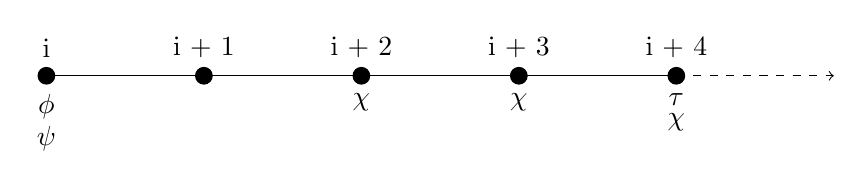
\begin{tikzpicture}
		      		\draw (1,0) -- (9,0);

		      		\filldraw (1,0) circle (3pt) node[below=3pt] {\shortstack{$\phi$ \\ $\psi$}} node[above=3pt] {i};
		      		\filldraw (3,0) circle (3pt) node[below=3pt] {} node[above=3pt] {i + 1};
		      		\filldraw (5,0) circle (3pt) node[below=3pt] {\shortstack{$\chi$}} node[above=3pt] {i + 2};
		      		\filldraw (7,0) circle (3pt) node[below=3pt] {\shortstack{$\chi$}} node[above=3pt] {i + 3};
		      		\filldraw (9,0) circle (3pt) node[below=3pt] {\shortstack{$\tau$ \\ $\chi$}} node[above=3pt] {i + 4};

		      		\draw[dashed, ->] (9,0) -- (11,0);
		      	\end{tikzpicture}
		      			      			      			      			      			      	
		      	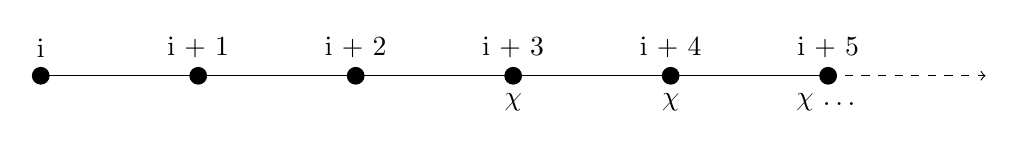
\begin{tikzpicture}
		      		\draw (1,0) -- (11,0);

		      		\filldraw (1,0) circle (3pt) node[below=3pt] {} node[above=3pt] {i};
		      		\filldraw (3,0) circle (3pt) node[below=3pt] {} node[above=3pt] {i + 1};
		      		\filldraw (5,0) circle (3pt) node[below=3pt] {} node[above=3pt] {i + 2};
		      		\filldraw (7,0) circle (3pt) node[below=3pt] {\shortstack{$\chi$}} node[above=3pt] {i + 3};
		      		\filldraw (9,0) circle (3pt) node[below=3pt] {\shortstack{$\chi$}} node[above=3pt] {i + 4};
		      		\filldraw (11,0) circle (3pt) node[below=3pt] {\shortstack{$\chi$} \ldots } node[above=3pt] {i + 5};

		      		\draw[dashed, ->] (11,0) -- (13,0);
		      	\end{tikzpicture}

                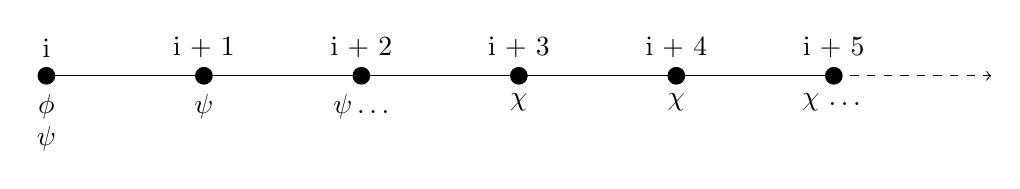
\begin{tikzpicture}
		      		\draw (1,0) -- (11,0);

		      		\filldraw (1,0) circle (3pt) node[below=3pt] {\shortstack{$\phi$ \\ $\psi$}} node[above=3pt] {i};
		      		\filldraw (3,0) circle (3pt) node[below=3pt] {$\psi$} node[above=3pt] {i + 1};
		      		\filldraw (5,0) circle (3pt) node[below=3pt] {$\psi \ldots$} node[above=3pt] {i + 2};
		      		\filldraw (7,0) circle (3pt) node[below=3pt] {\shortstack{$\chi$}} node[above=3pt] {i + 3};
		      		\filldraw (9,0) circle (3pt) node[below=3pt] {\shortstack{$\chi$}} node[above=3pt] {i + 4};
		      		\filldraw (11,0) circle (3pt) node[below=3pt] {\shortstack{$\chi$} \ldots } node[above=3pt] {i + 5};

		      		\draw[dashed, ->] (11,0) -- (13,0);
		      	\end{tikzpicture}

                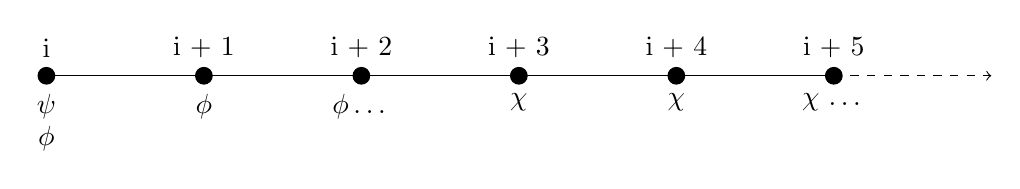
\begin{tikzpicture}
		      		\draw (1,0) -- (11,0);

		      		\filldraw (1,0) circle (3pt) node[below=3pt] {\shortstack{$\psi$ \\ $\phi$}} node[above=3pt] {i};
		      		\filldraw (3,0) circle (3pt) node[below=3pt] {$\phi$} node[above=3pt] {i + 1};
		      		\filldraw (5,0) circle (3pt) node[below=3pt] {$\phi \dots$} node[above=3pt] {i + 2};
		      		\filldraw (7,0) circle (3pt) node[below=3pt] {\shortstack{$\chi$}} node[above=3pt] {i + 3};
		      		\filldraw (9,0) circle (3pt) node[below=3pt] {\shortstack{$\chi$}} node[above=3pt] {i + 4};
		      		\filldraw (11,0) circle (3pt) node[below=3pt] {\shortstack{$\chi$} \ldots } node[above=3pt] {i + 5};

		      		\draw[dashed, ->] (11,0) -- (13,0);
		      	\end{tikzpicture}
		      \end{center}
		      		      		      		      		      		      
		      It should be noted that the requirement "none of $\phi$ or $\psi$ are invariants" introduces the idea that both atomic propositions $\phi$ and $\psi$ can be true at some point a finite number of times, and can also be false in other times as well.\\
		      		      		      		      		      		              
		      Additionally, with the lack of guarantee that the atomic proposition $\tau$ will ever become true, we can visualize the requirement as having the proposition become true at some point in time or simply never become true, letting the atomic proposition $\chi$ remain true.
		      		      		      		      		      		      
		\item (2 pts) Describe then visualize the following requirement: $(\neg \alpha \lor \neg \beta) \rightarrow \bigcirc \diamond (\gamma \: \mathcal{U} \: \delta)$\\
		      		      		      		      		      		      
		      \textbf{Solution}: We can describe and visualize the above requirement as follows:
		      		      		      		      		      		      
		      		      		      		      		      		              
		      \begin{itemize}
		      	\item If neither $\alpha$ nor $\beta$ is true, then at the next time instant, there exists a path where $\gamma$ holds until $\delta$ becomes true.
		      \end{itemize}
		      		      		      		      		      		      
		      \begin{center}
		      	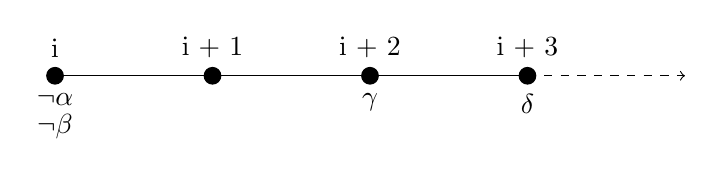
\begin{tikzpicture}
		      		\draw (1,0) -- (7,0);

		      		\filldraw (1,0) circle (3pt) node[below=3pt] {\shortstack{$\neg \alpha$ \\ $\neg \beta$}} node[above=3pt] {i};
		      		\filldraw (3,0) circle (3pt) node[below=3pt] {} node[above=3pt] {i + 1};
		      		\filldraw (5,0) circle (3pt) node[below=3pt] {\shortstack{$\gamma$}} node[above=3pt] {i + 2};
		      		\filldraw (7,0) circle (3pt) node[below=3pt] {\shortstack{$\delta$}} node[above=3pt] {i + 3};

		      		\draw[dashed, ->] (7,0) -- (9,0);
		      	\end{tikzpicture}t
		      			      			      			      			      			      	
		      	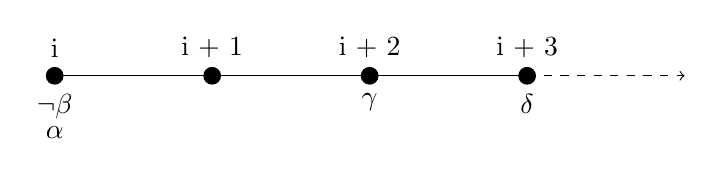
\begin{tikzpicture}
		      		\draw (1,0) -- (7,0);

		      		\filldraw (1,0) circle (3pt) node[below=3pt] {\shortstack{$\neg \beta$ \\ $\alpha$}} node[above=3pt] {i};
		      		\filldraw (3,0) circle (3pt) node[below=3pt] {} node[above=3pt] {i + 1};
		      		\filldraw (5,0) circle (3pt) node[below=3pt] {\shortstack{$\gamma$}} node[above=3pt] {i + 2};
		      		\filldraw (7,0) circle (3pt) node[below=3pt] {\shortstack{$\delta$}} node[above=3pt] {i + 3};

		      		\draw[dashed, ->] (7,0) -- (9,0);
		      	\end{tikzpicture}t
		      			      			      			      			      			      	
		      	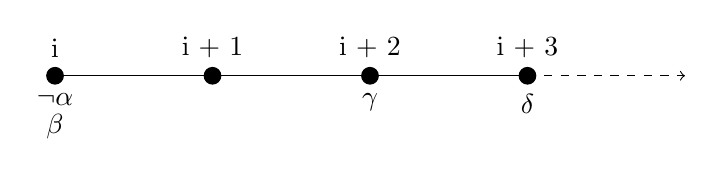
\begin{tikzpicture}
		      		\draw (1,0) -- (7,0);

		      		\filldraw (1,0) circle (3pt) node[below=3pt] {\shortstack{$\neg \alpha$ \\ $\beta$}} node[above=3pt] {i};
		      		\filldraw (3,0) circle (3pt) node[below=3pt] {} node[above=3pt] {i + 1};
		      		\filldraw (5,0) circle (3pt) node[below=3pt] {\shortstack{$\gamma$}} node[above=3pt] {i + 2};
		      		\filldraw (7,0) circle (3pt) node[below=3pt] {\shortstack{$\delta$}} node[above=3pt] {i + 3};

		      		\draw[dashed, ->] (7,0) -- (9,0);
		      	\end{tikzpicture}t
		      \end{center}
		      		      		      		      		      		      
		      		      		      		      		      		      
		\item (2 pts) Describe then visualize the following requirement: $(\bigcirc \tau \land \bigcirc \diamond \square \chi) \rightarrow \bigcirc^2 (\phi \: \mathcal{W} \: \psi )$\\
		      		      		      		      		      
		      \textbf{Solution}: We can describe and visualize the above requirement as follows:
		      		      		      		      		      		      
		      		      		      		      		      		              
		      \begin{itemize}
		      	\item  If at the next time instant $\tau$ holds and at some future time there exists a path where $\chi$ is invariant, then two time steps later, $\phi$ will remain true until $\psi$ becomes true. There is no guarantee that $\psi$ will become true.
		      \end{itemize}
		      		      		      		      		      
		      \begin{center}
		      	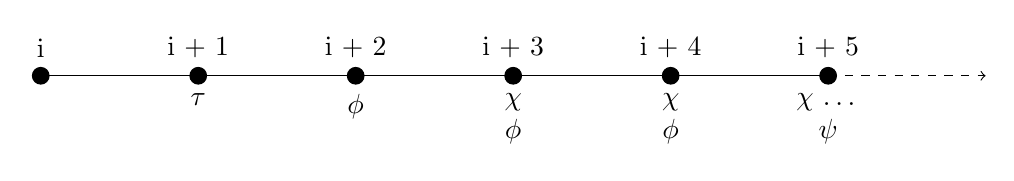
\begin{tikzpicture}
		      		\draw (1,0) -- (11,0);

		      		\filldraw (1,0) circle (3pt) node[below=3pt] {} node[above=3pt] {i};
		      		\filldraw (3,0) circle (3pt) node[below=3pt] {\shortstack{$\tau$}} node[above=3pt] {i + 1};
		      		\filldraw (5,0) circle (3pt) node[below=3pt] {\shortstack{$\phi$}} node[above=3pt] {i + 2};
		      		\filldraw (7,0) circle (3pt) node[below=3pt] {\shortstack{$\chi$ \\ $\phi$}} node[above=3pt] {i + 3};
		      		\filldraw (9,0) circle (3pt) node[below=3pt] {\shortstack{$\chi$ \\$\phi$}} node[above=3pt] {i + 4};
		      		\filldraw (11,0) circle (3pt) node[below=3pt] {\shortstack{$\chi$ \ldots \\ $\psi$}} node[above=3pt] {i + 5};

		      		\draw[dashed, ->] (11,0) -- (13,0);
		      	\end{tikzpicture}
		      			      			      			      			      	
		      	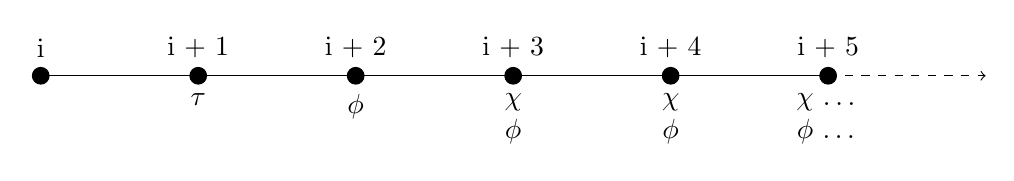
\begin{tikzpicture}
		      		\draw (1,0) -- (11,0);

		      		\filldraw (1,0) circle (3pt) node[below=3pt] {} node[above=3pt] {i};
		      		\filldraw (3,0) circle (3pt) node[below=3pt] {\shortstack{$\tau$}} node[above=3pt] {i + 1};
		      		\filldraw (5,0) circle (3pt) node[below=3pt] {\shortstack{$\phi$}} node[above=3pt] {i + 2};
		      		\filldraw (7,0) circle (3pt) node[below=3pt] {\shortstack{$\chi$ \\ $\phi$}} node[above=3pt] {i + 3};
		      		\filldraw (9,0) circle (3pt) node[below=3pt] {\shortstack{$\chi$ \\$\phi$}} node[above=3pt] {i + 4};
		      		\filldraw (11,0) circle (3pt) node[below=3pt] {\shortstack{$\chi$ \ldots \\ $\phi$ \ldots}} node[above=3pt] {i + 5};

		      		\draw[dashed, ->] (11,0) -- (13,0);
		      	\end{tikzpicture}
		      \end{center}
		      		      		      		      		        
	\end{enumerate}	    
	\newpage
	\section*{PROBLEM 4: Unordered Structures (14 pts)}
					
	Consider the following set:
				
	$Languages=Ruby, Go, Lisp, Rust, C, Groovy, Python, Clojure, \{Lua, Groovy, C\}$\\
				
	Answer the following questions:
				
	\begin{enumerate}
		\item (1 pt) Provide a description (in plain English) on what is meant by $\mathcal{P} \: Languages$.
		      		      		      		      
		      \textbf{Answer:} The set $\mathcal{P} Languages$ refers to the power set of the set "Languages." In plain English, the power set of a set is the set of all possible subsets that can be formed from the original set. In this context, $\mathcal{P} Languages$ would represent all possible combinations of subsets that can be created from the set of languages provided, including the empty set, individual languages, and combinations of multiple languages.\\
		      		      		      		      
		\item (1 pt) Describe it in detail (a) what the expression $Favorites\: : \: \mathcal{P} \: Languages$ signifies and (b) how it should be interpreted. (c) What would be any legitimate value for variable $Favorites$?
		      		      		      		      
		      \begin{enumerate}
		      	\item The expression $Favorites : \mathcal{P} Languages$ signifies that the variable $Favorites$ is associated with the power set of the set "Languages." This means that $Favorites$ can take on values that are subsets of the set of languages provided, including all possible combinations of languages within the set. 
		      	      		      	      		      	      		      	                      
		      	\item The expression should be interpreted as allowing the variable $Favorites$ to represent any subset of languages from the given set "Languages." It provides flexibility for $Favorites$ to encompass various combinations of programming languages, including individual languages, multiple languages, or even an empty set. 
		      	      		      	      		      	      		      	                      
		      	\item Legitimate values for the variable $Favorites$ could include any subset of the languages listed in the set "Languages," such as individual languages like Ruby or Python, combinations like {Ruby, Go}, or even the empty set if no language is selected as a favorite.
		      \end{enumerate}
		      		      		      		      
		\item (1 pt) What does the expression $Favorites = \mathcal{P} \: Languages$ signify and (b) Is it semantically equivalent to $Favorites \: : \: \mathcal{P} \: Languages$?
		      		      		      		      
		      \begin{enumerate}
		      	\item The expression $Favorites = \mathcal{P} \: Languages$ signifies that the variable $Favorites$ is assigned the value of the power set of the set "Languages." This means that $Favorites$ represents all possible subsets that can be formed from the original set of languages provided. 
		      	      		      	      		      	      		      	                      
		      	\item Semantically, $Favorites = \mathcal{P} \: Languages$ and $Favorites : \mathcal{P} \: Languages$ are not equivalent. The former indicates that the variable $Favorites$ is set to be equal to the power set of languages, implying a specific assignment of values. On the other hand, the latter notation suggests a relationship or association between $Favorites$ and the power set of languages without explicitly assigning a specific value.\\
		      \end{enumerate}
		      		      		      		                  
		\item (1 pt) Is $\{Lua, Groovy, C\} \in \mathcal{P} \: Languages$? Explain in detail.
		      		      		      		      
		      \textbf{Answer:} The expression $\{Lua, Groovy, C\} \in \mathcal{P} \: Languages$ signifies whether the set $\{Lua, Groovy, C\}$ is an element of the power set of the set "Languages." In detail, the power set of a set contains all possible subsets of that set, including the empty set and the set itself. Therefore, for $\{Lua, Groovy, C\}$ to be in the power set of "Languages," it must be a valid subset that can be formed from the original set of languages provided.\\
		      		      		      		                  
		      In this case, since $\{Lua, Groovy, C\}$ is a specific combination of languages from the set "Languages," it is indeed an element of the power set. This is because any subset that can be formed from the original set, including combinations of languages like $\{Lua, Groovy, C\}$, is considered part of the power set.\\
		      		      		      		                  
		\item (1 pt) Is $\{\{Lua, Groovy, C\}\} \subset \mathcal{P} \: Languages$? Explain in detail.
		      		      		      		      
		      \textbf{Answer:}  The expression $\{\{Lua, Groovy, C\}\} \subset \mathcal{P} \: Languages$ signifies whether the set $\{\{Lua, Groovy, C\}\}$ is a subset of the power set of the set "Languages." In detail, a subset is a set that contains only elements that are also in another set. The power set of a set contains all possible subsets that can be formed from the original set.\\
		      		      		      		                  
		      In this case, the set $\{\{Lua, Groovy, C\}\}$ is not a subset of the power set of "Languages" because the power set includes all possible combinations of subsets of the original set. The element $\{\{Lua, Groovy, C\}\}$ is a nested set within itself and does not directly match any subset that can be formed from the original set of languages provided.\\
		      		      		      		                  
		\item (1 pt) What is the difference between the following two variable declarations and are the two variables atomic or non-atomic?
		      		      		      		                  
		      \begin{enumerate}
		      	\item $\lambda_1 : Languages$
		      	      		      	      		      	      		      	      
		      	      \textbf{Answer:} This variable declaration $\lambda_1$ signifies that it is associated with the set "Languages." Here, $\lambda_1$ can take on values directly from the set of languages provided. The variable $\lambda_1$ is atomic as it directly refers to individual elements within the set "Languages."\\
		      	      		      	      		      	      		      	                  
		      	\item $\lambda_2 : \mathcal{P} \: Languages$
		      	      		      	      		      	      		      	          
		      	      \textbf{Answer:} In contrast, the variable declaration $\lambda_2$ indicates that it is linked to the power set of the set "Languages." This means that $\lambda_2$ can represent any subset that can be formed from the original set of languages. The variable $\lambda_2$ is non-atomic as it encompasses various combinations and subsets of languages rather than individual elements directly from the set.\\
		      	      		      	      		      	      		      	                  
		      \end{enumerate}
		      		      		      		      
		\item (1 pt) In the expression $Library = \{C, Ruby, Go\}$ where the variable is used to hold any collection that can be constructed from $Languages$, what is the \textit{type} of the variable?
		      		      		      		      
		      \textbf{Answer:} The type of the variable in the expression $Library = {C, Ruby, Go}$, where it is used to hold any collection that can be constructed from $Languages$, would typically be an array or a list in programming languages like Ruby. The variable $Library$ is intended to store a collection of programming languages, and using an array or list data structure would allow for easy manipulation and access to these languages within the collection.\\
		      		      		      		                  
		\item (1 pt) Is $\{\varnothing\} \in \mathcal{P} \: Languages$? Explain.
		      		      		      		      
		      \textbf{Answer:} The set $\{\varnothing\}$ is indeed an element of the power set of the set "Languages." This is because the power set includes all possible subsets that can be formed from the original set, including the empty set. Since $\{\varnothing\}$ represents a subset that contains only the empty set, it is a valid element of the power set of "Languages."\\
		      		      		      		                  
		\item (6 pts) (\textbf{\uline{{PROGRAMMING}}}) Use Common LISP to implement the functions below and demonstrate the behavior of each function with a listing of your interaction with the language environment. \textbf{Do not use imperative constructs}.
		      		      		      		      
		      \begin{itemize}
		      	\item \textbf{is-memberp} Returns true if its first argument is found to be a member in the set provided by the second argument. Returns nil (false) otherwise.

                    \lstinputlisting[language=Lisp]{code/is-member_4_9.lisp}
		      	      		      	      		      	      		      	                      
		      	\item \textbf{equal-setsp} Returns true if its two arguments are two identical sets. Returns nil (false) otherwise. You may assume that neither argument (set) contains any redundancies.

                    \lstinputlisting[language=Lisp]{code/equal-setsp_4_9.lisp}
		      	      		      	      		      	      		      	                      
		      \end{itemize}
		      		      		      		                  
	\end{enumerate}
				        
	\newpage
	\section*{PROBLEM 5: Ordered Structures (15 pts)}
	Consider the Queue Abstract Data Type (ADT), $\mathbb{Q}$, defined over some generic type $\mathbb{T}$ and defined using two stacks, $\sum_1$ and $\sum_2$, where a Stack ADT is implemented as a list, $\Lambda$. (\textit{Hint: } This description implies that the only available operations are those defined for a list.) 
				
	\begin{enumerate}
		\item (10 pts) Define operations \textit{Enqueue}$(\mathbb{Q},\mathbb{T})$ and \textit{Dequeue}$(\mathbb{Q})$
		      		      		      		      
		      \textbf{Solution}: To enqueue an element of type $\mathbb{T}$ into the queue $\mathbb{Q}$:
		      		      		      		      
		      \begin{enumerate}
		      	\item We simply add the element to one of the stacks (let's say $\sum_1$).
		      	\item There's no need to consider the contents of the other stack for this operation.
		      	\item This operation corresponds to appending the element to the end of the list representing $\sum_1$.
		      \end{enumerate} 
		      		      		      		      
		      To dequeue an element from the queue $\mathbb{Q}$:
		      		      		      		      
		      \begin{enumerate}
		      	\item If $\sum_2$ is not empty, we pop and return the top element from $\sum_2$.
		      	\item If $\sum_2$ is empty:
		      	      \begin{itemize}
		      	      	\item We transfer all elements from $\sum_1$ to $\sum_2$, effectively reversing their order.
		      	      	\item Then, we pop and return the top element from $\sum_2$.
		      	      \end{itemize}
		      	\item This operation involves transferring elements between stacks to maintain the FIFO (First-In-First-Out) order.
		      	\item This corresponds to removing the last element from the list representing $\sum_2$.
		      \end{enumerate}
		      		      		      		      
		      To better visualize the operations, we can imagine the following scenario:
		      		      		      		      
		      Let's imagine managing a queue at a ticket counter. Initially, there are two empty stacks, one for incoming tickets and the other for processing them. Enqueueing involves adding tickets to the incoming stack. For instance, when the first three tickets arrive (let's say labeled A, B, and C, in that particular order), they are placed in the incoming stack in reverse order, so A is at the bottom and C is at the top.
		      		      		      		              
		      When it's time to serve a customer, we transfer tickets from the incoming stack to the processing stack, ensuring we serve the oldest ticket first. In this case, we transfer tickets from the incoming stack to the processing stack, so now the processing stack holds tickets A, B, and C in the desired, "queue-like", order (FIFO). We serve ticket A first, transferring it out of the processing stack.
		      		      		      		              
		      Subsequent tickets are added to the incoming stack, maintaining the queue order. When we serve a ticket, we remove it from the processing stack, ensuring the next ticket served is the next in line. This process continues, ensuring that tickets are served in the order they were received. Tickets from the incoming stack are only sent to the processing stack when the processing stack is empty.
		      		      		      		      
		\item (3 pts) (\textbf{\uline{PROGRAMMING}}) Use Common LISP to define two stacks (\texttt{stack1} and \texttt{stack2} as global variables to hold the collection, and implement functions \texttt{enqueue} and \texttt{dequeue}.

            \lstinputlisting[language=Lisp]{code/enqueue-dequeue_5_2.lisp}
		      		      		      		              
		\item (2 pts) (\textbf{\uline{PROGRAMMING}}) Implement operations \textit{head}, \textit{tail} and \textit{cons} in Prolog and demonstrate their usage.

            \lstinputlisting[language=Prolog]{code/head-tail-cons_5_3.pl}
		      		      		      
		      \begin{enumerate}
		      	\item \textbf{head/2}: This predicate retrieves the first element of a list. It takes a list as its first argument and a variable to unify with the first element of the list. In Prolog, lists are represented as nested pairs [Head$|$Tail], where Head is the first element and Tail is the rest of the list. The head/2 predicate pattern-matches the list [Head$|$\_] and unifies Head with the first element of the list.
		      	      		      	      		      	      
		      	\item \textbf{tail/2}: This predicate returns the list without its first element. Similarly to head/2, it also takes a list as its first argument and a variable to unify with the tail of the list. It pattern-matches the list [\_$|$Tail], ignoring the first element and unifying Tail with the remaining elements of the list.
		      	      		      	      		      	      
		      	\item \textbf{cons/3}: This predicate adds an element to the beginning of a list. It takes three arguments: an element to add, an existing list, and a variable to unify with the resulting list. It constructs a new list by prepending the given element to the existing list, resulting in [Element$|$List]. This predicate is commonly used to build lists recursively in Prolog.
		      \end{enumerate}
		      		      		      
		      Here are some queries that test the above Prolog predicates:
		      		      		      
		      \begin{enumerate}
		      	\item Query to get the first element of a list:
		      	      \begin{itemize}
		      	      	\item \textbf{Input:} \texttt{head([1,2,3,4], X).}
		      	      	\item \textbf{Output:} \texttt{X = 1} 
		      	      \end{itemize}
		      	      		      	      		      	      
		      	\item Query to get the tail of a list:
		      	      \begin{itemize}
		      	      	\item \textbf{Input:} \texttt{tail([1,2,3,4], X).}
		      	      	\item \textbf{Output:} \texttt{X = [2, 3, 4]} 
		      	      \end{itemize}
		      	      		      	      		      	      
		      	\item Query to add an element to the beginning of a list:
		      	      \begin{itemize}
		      	      	\item \textbf{Input:} \texttt{cons(5, [1,2,3,4], X).}
		      	      	\item \textbf{Output:} \texttt{X = [5, 1, 2, 3, 4]} 
		      	      \end{itemize}
		      \end{enumerate}
		      		      		      		      
	\end{enumerate}
				     
	\newpage
	\section*{PROBLEM 6: Binary Relations, Functions and Orderings (20 pts)}
			
	\textbf{Part 1} (6 pts)
			
	\begin{enumerate}
		\item (2 pts) Consider the binary relation $R$: "is of type" in the domain of types in the Java API. Prove that $R$ is \textit{a partial order}.
		      		      		      
		      \textbf{Solution:} To prove that the binary relation $R$: "is of type" in the domain of types in the Java API is a partial order, we need to show that it satisfies three properties: reflexivity, antisymmetry, and transitivity.
		      		      		      
		      \begin{enumerate}
		      	\item \textbf{Reflexivity:}
		      	      \begin{itemize}
		      	      	\item For any type $T$, $T$ is of type $T$. This property holds as every type is of its own type.
		      	      \end{itemize}
		      	      		      	      		      	      
		      	\item \textbf{Antisymmetry:}
		      	      \begin{itemize}
		      	      	\item If $T_1$ is of type $T_2$ and $T_2$ is of type $T_1$, then $T_1 = T_2$. This property holds as types are uniquely defined.
		      	      \end{itemize}
		      	      		      	      		      	      
		      	\item \textbf{Transitivity:}
		      	      \begin{itemize}
		      	      	\item If $T_1$ is of type $T_2$ and $T_2$ is of type $T_3$, then $T_1$ is of type $T_3$. This property holds as types can be hierarchically related.
		      	      \end{itemize}
		      \end{enumerate}
		      		      		      
		      Therefore, the binary relation $R$: "is of type" in the domain of types in the Java API satisfies reflexivity, antisymmetry, and transitivity, making it a partial order. 
		      		      		      
		\item (2 pts) Given the set of vertices
		      		      		      
		      \begin{align*}
		      	V_1= \{ & Dictionary, TreeMap, SortedMap, AbstractMap, Hashtable, \\
		      	        & LinkedHashMap, Map, NavigableMap, HashMap\}             
		      \end{align*}
		      		      		              
		      and the set of edges
		      		      		      
		      \begin{align*}
		      	E = \{ & (LinkedHashMap, HashMap), (HashMap, AbstractMap), (Hashtable, Dictionary),  \\
		      	       & (TreeMap, AbstractMap), (TreeMap, NavigableMap), (NavigableMap, SortedMap), \\
		      	       & (Hashtable, Map), (AbstractMap, Map), (SortedMap, Map) \}                   
		      \end{align*}
		      		      		      
		      Prove that $(V_1, R)$ is a \textit{poset}.
		      		      		      
		      \textbf{Solution}:  To demonstrate that the set $(V_1, R)$ is a poset, we first establish that the binary relation $R$ ("is of type") is a partial order. This involves verifying three key properties: reflexivity, antisymmetry, and transitivity.
		      		      
		      \begin{itemize}
		      	\item Reflexivity: Every type is inherently of its own type, ensuring that the relation is reflexive.
		      	      		      	              
		      	\item Antisymmetry: The relation between types is uniquely defined, preventing two distinct types from being of each other's type.
		      	      		      	              
		      	\item Transitivity: Types can be hierarchically related, allowing for the transitive property to hold.
		      	      		      	              
		      \end{itemize} 
		      		      
		      Having confirmed that $R$ is a partial order, we proceed to analyze the set of vertices and edges provided. By constructing a directed acyclic graph based on these elements, we observe that the graph maintains acyclicity. This acyclic nature aligns with the requirements of a partial order set, reinforcing the poset structure of $(V_1, R)$. 
		      		                  
		      Therefore, through the fulfillment of partial order properties and the absence of cycles in the directed graph representing $(V_1, R)$, we can confidently assert that this set forms a poset.       
		      		      		              
		\item (2 pts) Create a Hasse Diagram to visualize $V, R$ and identify \textit{maximal} and \textit{minimal} elements.
		      		      
		      \begin{figure}[htp]
		      	\centering
		      	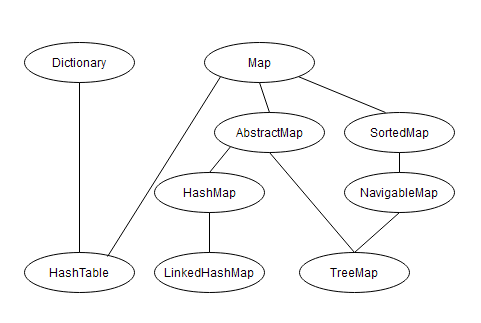
\includegraphics{static/HasseDiagram_6_3_1.png}
		      	\caption{Hasse Diagram Depicting $(V_1,R)$}
		      	\label{fig:figure}
		      \end{figure}
		      		           
		      \begin{itemize}
		      	\item \textbf{Minimal Elements}: $HashTable$, $LinkedHashMap$ and $TreeMap$
		      	\item \textbf{Maximal Elements}: $Dictionary$ and $Map$
		      \end{itemize}
		      		      		      
	\end{enumerate}
			
	\noindent \textbf{Part 2} (6 pts)
			
	\begin{enumerate}
		\item (2 pts) Consider the binary relation $\subseteq$: "is subset of" in the domain of sets. Prove that $\subseteq$ is a partial order.
		      		      
		      To prove that the binary relation $\subseteq$ ("is subset of") in the domain of sets is a partial order, we need to demonstrate three key properties: reflexivity, antisymmetry, and transitivity.
		      		      
		      \begin{itemize}
		      	\item \textbf{Reflexivity}: Every set is a subset of itself, satisfying the reflexivity property.
		      	      		      	      
		      	\item \textbf{Antisymmetry}: If set $A$ is a subset of set $B$ and $B$ is a subset of $A$, then $A = B$, ensuring antisymmetry.
		      	      		      	      
		      	\item \textbf{Transitivity}: If set $A$ is a subset of set $B$ and $B$ is a subset of set $C$, then $A$ is also a subset of $C$, validating transitivity.
		      \end{itemize}
		      		      
		      Since $\subseteq$ fulfills these properties, it qualifies as a partial order.
		      		      
		\item (2 pts) Given the set $V_2=\{a,b,c\}$, prove that $(\mathcal{P}(V_2),\subseteq)$ is a poset.
		      		      
		      \textbf{Solution}: To prove that the relation $\subseteq$ applied over the set $V_2=\{a,b,c\}$ is a poset, we need to demonstrate three key properties: reflexivity, antisymmetry, and transitivity.
		      		              
		      \begin{itemize}
		      	\item \textbf{Reflexivity:}
		      	      For any set \( S \) in \( \mathcal{P}(V_2) \), we have \( S \subseteq S \) since every set is a subset of itself. Therefore, \( (\mathcal{P}(V_2),\subseteq) \) is reflexive.
		      	      		      	                  
		      	\item \textbf{Antisymmetry:}
		      	      If \( A \subseteq B \) and \( B \subseteq A \) for sets \( A \) and \( B \) in \( \mathcal{P}(V_2) \), then \( A = B \). This is true because two sets are equal if and only if they contain the same elements. Therefore, \( (\mathcal{P}(V_2),\subseteq) \) is antisymmetric.
		      	      		      	                  
		      	\item \textbf{Transitivity:}
		      	      If \( A \subseteq B \) and \( B \subseteq C \) for sets \( A \), \( B \), and \( C \) in \( \mathcal{P}(V_2) \), then \( A \subseteq C \). This is true because if every element of \( A \) is in \( B \) and every element of \( B \) is in \( C \), then every element of \( A \) is also in \( C \). Therefore, \( (\mathcal{P}(V_2),\subseteq) \) is transitive.
		      \end{itemize}
		      		              
		      Since \( (\mathcal{P}(V_2),\subseteq) \) satisfies reflexivity, antisymmetry, and transitivity, it is a poset.
		      		              
		\item (2 pts) Create a Hasse Diagram to visualize $(\mathcal{P}(V_2),\subseteq)$ and identify \textit{maximal} and \textit{minimal} elements.

            \textbf{Solution}: The maximal and minimal elements of the diagram are \textit{a,b,c} and $\{\varnothing\}$, respectively.
            
		      \begin{figure}[htp]
		      	\centering
		      	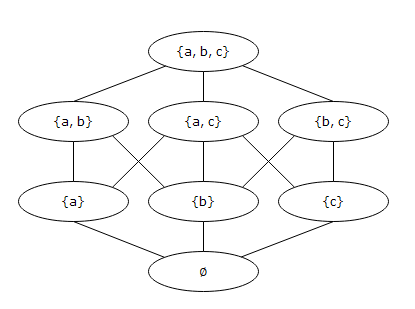
\includegraphics{static/HasseDiagram_6_2_3.png}
		      	\caption{Hasse Diagram Depicting $(\mathcal{P}(V_2),\subseteq)$}
		      	\label{fig:figure}
		      \end{figure}
		      		        
	\end{enumerate}
			    
	\noindent \textbf{Part 3} (8 pts)
			
	\noindent Consider $(V_1, R)$ and $(\mathcal{P}(V_2), \subseteq)$ from Parts 1 and 2 respectively. Assume the following mapping, captured by variable \textit{map}:
			
	\begin{align*}
		map = \{ & Dictionary \mapsto \{a,b,c\},  \\
		         & AbstractMap \mapsto \{a,b,c\}, \\
		         & NavigableMap \mapsto \{c\},    \\
		         & TreeMap \mapsto \varnothing\}  
	\end{align*}
			
	\noindent Is \textit{map} a function? Discuss \textbf{in detail} (in plain English \uline{and} formally) all applicable properties (total vs. partial function, injectivity, surjectivity, bijection, order preserving, order reflecting, order embedding, isomorphism).\\
		
	\begin{figure}[htp]
		\centering
		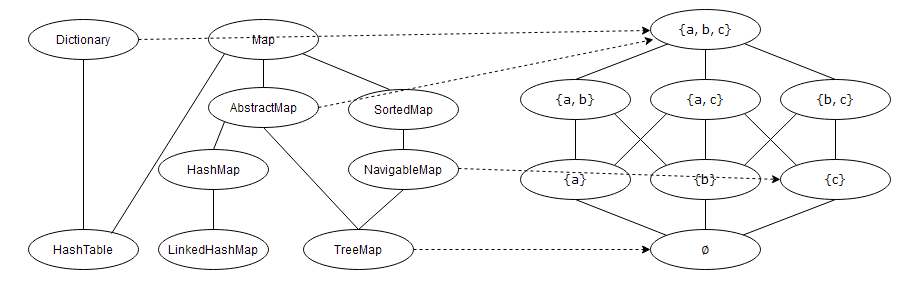
\includegraphics[width=1.1\textwidth]{static/FunctionMapping_6_3.png}
		\caption{Function $map$}
		\label{fig:figure}
	\end{figure}
		
	\noindent \textbf{Solution}: The variable \textit{map} captures a mapping between elements in $(V_1, R)$ and subsets in $(\mathcal{P}(V_2), \subseteq)$. Let's evaluate whether \textit{map} qualifies as a function and explore various properties it exhibits.\\
		
	\noindent We begin by defining the various properties of a function in plain English:
		
	\begin{itemize}
		\item \textbf{Functionality}: A function assigns each element from the domain to exactly one element in the codomain.
		      		              
		\item \textbf{Total vs. Partial Function}: A total function maps every element from the domain to an element in the codomain, while a partial function may not cover all elements.
		      		          
		\item \textbf{Injectivity}: An injective function ensures distinct elements in the domain map to distinct elements in the codomain.
		      		          
		\item \textbf{Surjectivity}: A surjective function covers every element in the codomain.
		      		          
		\item \textbf{Bijection}: A bijective function is both injective and surjective, establishing a one-to-one correspondence.
		      		          
		\item \textbf{Order Preservation}: Preserving order means that if $a < b$ in the domain, then $f(a) < f(b)$ in the codomain.
		      		          
		\item \textbf{Order Reflection}: Reflecting order implies that if $f(a) < f(b)$ in the codomain, then $a < b$ in the domain.
		      		          
		\item \textbf{Order Embedding}: A function is order-embedding if it is both order-preserving and order-reflecting.
		      		          
		\item \textbf{Isomorphism}: A function that is order-embedding and surjective is called isomorphic. 
	\end{itemize}
		
	\noindent We can now perform a formal analysis using the definitions of the properties that we are working with:
		
	\begin{itemize}
		\item \textbf{Functionality Check}: For each element in $(V_1, R)$, \textit{map} assigns a unique subset from $(\mathcal{P}(V_2), \subseteq)$, meeting the function criteria.
		      		      
		\item \textbf{Total vs. Partial Function}: \textit{map} is a partial function since not all elements from $(V_1, R)$ are mapped to subsets in $(\mathcal{P}(V_2), \subseteq)$.
		      		      
		\item \textbf{Injectivity}: Since multiple elements from $(V_1, R)$ map to $\{a,b,c\}$, \textit{map} is not injective.
		      		      
		\item \textbf{Surjectivity}: Not every subset of the power set of $\{a,b,c\}$ are mapped to elements in the domain, $(V_1,R)$. \textit{map} is not surjective.
		      		      
		\item \textbf{Bijection}: As \textit{map} is not injective nor surjective, it cannot be bijective.
		      		      
		\item \textbf{Order Preservation/Reflection/Embedding}: The mapping does not reflect or preserve any order relationships between elements of $(V_1, R)$ or subsets of $(\mathcal{P}(V_2), \subseteq)$.
		      		      
		\item \textbf{Isomorphism}: Since \textit{map} is neither order-embedding nor surjective, it cannot be isomorphic.
	\end{itemize}
		
	\noindent In summary, while \textit{map} functions as a partial function and exhibits surjectivity for certain subsets, it lacks properties like injectivity and order preservation/reflection necessary for bijection or isomorphism.
			    
	\newpage
	\section*{PROBLEM 7: Construction Techniques (10 pts)}
		
	Define a function $compress : lists(\mathbb{T}) \rightarrow lists(\mathbb{T})$ that accepts a list argument (of some generic type $\mathbb{T}$) and returns a list without any \textit{subsequent} redundancies.
		
	\begin{enumerate}
		\item (2 pts) Transform the definition into a computable function.
		      		      
		      We transform the definition of $compress$ into a computable function using available operations on the underlying structure (list).
		      
		      We can use \texttt{cons} as follows:
		      
		      $$\text{compress}(lst) =\begin{cases}\text{[]}, & \text{if } lst = \text{[]} \\\text{[x]}, & \text{if } \text{length}(lst) = 1 \text{ where } lst = \text{[x]} \\\text{cons}(x, \text{compress}(y)), & \text{otherwise where } lst = \text{x:y} \text{ (head:tail) and } x \neq \text{head}(y) \\\text{compress}(y), & \text{otherwise where } lst = \text{x:y} \text{ (head:tail) and } x = \text{head}(y) \\\end{cases}$$
		      		
		\item (3 pts) Define $f$ recursively.
		      		      
		      To define the function $f$ recursively for compressing a list without subsequent redundancies, we can express it as follows: 
		      		      
		      \begin{itemize}
		      	\item Let $L = [a_1, a_2, ..., a_n]$ be a list of elements of some generic type $\mathbb{T}$.
		      	      		      	      
		      	\item The function $f(n)$ recursively compresses the list to remove subsequent redundancies.
		      \end{itemize}
		      		      
		      The recursive definition of function $f$ can be outlined as: 
		      		      
		      \begin{enumerate}
		      	\item \textbf{Base Case}: 
		      	      \begin{itemize}
		      	      	\item If the list is empty, then $f(n) = []$, as an empty list has no subsequent redundancies.
		      	      	      		      	      	                          
		      	      	\item If $n = 1$, then $f(n) = [a_1]$, as a single-element list has no subsequent redundancies.
		      	      \end{itemize}
		      	      		      	      
		      	\item \textbf{Recursive Steps}:
		      	      \begin{itemize}
		      	      	\item If $a_n = a_{n-1}$, then $f(n) = f(n-1)$, as the current element is redundant.
		      	      	      		      	      	      
		      	      	\item If $a_n \neq a_{n-1}$, then $f(n) = f(n-1) \cup [a_n]$, adding the current element to the compressed list.
		      	      \end{itemize}
		      \end{enumerate}
		      		      
		\item (2 pts) Unfold your definition for $compress(\langle a, a, b, b, c, a \rangle)$.
		      		      
		      Let's unfold the recursive definition of the function $compress$ for the input list $\langle a, a, b, b, c, a \rangle$ step by step:
		      		      
		      \begin{enumerate}
		      	\item Initial List: $\langle a, a, b, b, c, a \rangle$
		      	      		      	      
		      	\item $f(1) = \langle a \rangle$ (Base case: First element is added to the compressed list)
		      	      		      	      
		      	\item $f(2) = f(1) = \langle a \rangle$ (Skipping the subsequent redundant element)
		      	      		      	      
		      	\item $f(3) = f(2) \cup \langle b \rangle = \langle a \rangle \cup \langle b \rangle = \langle a, b \rangle$ (Adding the non-redundant element)
		      	      		      	      
		      	\item $f(4) = f(3) = \langle a, b \rangle$ (Skipping the subsequent redundant element)
		      	      		      	      
		      	\item $f(5) = f(4) \cup \langle c \rangle = \langle a, b \rangle \cup \langle c \rangle = \langle a, b, c \rangle$ (Adding the non-redundant element)
		      	      		      	      
		      	\item $f(6) = f(5) \cup \langle a \rangle = \langle a, b, c \rangle \cup \langle a \rangle = \langle a, b, c, a \rangle$ (Adding the last non-redundant element)\\
		      \end{enumerate}
		      
		      Alternatively, we can unfold the computable definition of the function as well,
		      
		      \begin{enumerate}
		      	\item Initial List: $\langle a, a, b, b, c, a \rangle$
		      	      \begin{align*}
		      	      	compress(\langle a, a, b, b, c, a \rangle) & = cons(a, compress(\langle a, b, b, c, a \rangle))       \\
                           & = cons(a, cons(b, compress(\langle b, c, a \rangle)))    \\
                           & = cons(a, cons(b, cons(c, compress(\langle a \rangle)))) \\
                           & = cons(a, cons(b, cons(c, a)))                           \\
                           & = \langle a, b, c, a \rangle                             
		      	      \end{align*}
		      	                      
		      \end{enumerate}
		      		      
		\item (3 pts) (\uline{\textbf{PROGRAMMING}} Map your definition into a Common LISP function.\\
            
            \lstinputlisting[language=Lisp]{code/compress_7_4.lisp}	          
		      		              
	\end{enumerate}
\end{spacing}
\end{document}